
\documentclass[10 pt,letterpaper]{article}

\RequirePackage{bibentry}
\makeatletter\let\saved@bibitem\@bibitem\makeatother

\usepackage{mathptmx}
\usepackage{enumitem}
\usepackage{fancyhdr}
\usepackage{svg}
\usepackage{amsmath}
\usepackage{float}
\usepackage{colortbl}
\usepackage[labelfont=bf]{caption}
\usepackage{xcolor}
\usepackage{hyperref}
\hypersetup{colorlinks=true,urlcolor=teal,citecolor=teal,linkcolor=red}
\hypersetup{
	colorlinks=true,
	linkcolor=red,
	citecolor={green!60!blue},
	urlcolor=teal
}
\usepackage{multirow}
\usepackage{apacite}
\usepackage[sc]{mathpazo}

\usepackage[top=1in, bottom=1in, left=1.333in, right=1.333in]{geometry}
\renewcommand{\baselinestretch}{1.11} 

\pagestyle{fancy}
\fancyhf{}
\renewcommand{\headrulewidth}{0pt}
\fancyfoot[C]{(\thepage)}
\setlength{\parskip}{\baselineskip}%
\setlength{\parindent}{0pt}%


\title{
	Inequalities of extreme commuting across Canada
} 
\date{
	\today}


\begin{document}


\LARGE
\textsf{\textbf{Inequalities of extreme commuting across Canada}}

\vspace{4mm}


	\large
	
	Jeff Allen$^{*,1}$, Matthew Palm$^{2}$, Ignacio Tiznado-Aitken$^{2}$, Steven Farber$^{2}$

	\normalsize
	
	$^{*}$Corresponding Author (\url{jeff.allen@utoronto.ca})
	
	
	$^{1}$Department of Geography \& Planning, 
	University of Toronto, Canada
	\\
	$^{2}$Department of Human Geography, University of Toronto Scarborough, Canada
	
	
	
	
	
	\subsection*{{Abstract:}}
	
	\vspace{-5mm}
	
	There is growing body of research and practice assessing transportation equity and justice. Commuting is an especially important dimension to study since such frequent, non-discretionary travel, can come at the expense of time for other activities and therefore negatively impact mental health and well-being. An "extreme commuter" is a worker who has a particularly burdensome commute, and has previously been defined based on one-way commute times above 60 or 90 minutes. In this paper, we examine the social and geographic inequalities of extreme commuting in Canada. We use a 25\% sample of all commuters in Canada in 2016 ($n$ = 4,543,417) and our analysis consists of descriptive statistics and logistic regression models. The average one-way commute time in 2016 across Canada was 26 minutes, but over 9.7\% of the workforce had commute times exceeding 60 minutes. However, this rate of extreme commuting was 11.5\% for low-income households, 13.5\% for immigrants, and 13.4\% among non-white Canadians, reaching as high as 18.6\% for Black Canadians and 14.7\% for Latin American Canadians specifically. We find that these inequalities persist even after controlling for household factors, commute mode, occupation, and built environment characteristics. The persistently significant effects of race in our models point to factors like housing and employment discrimination as possible contributors to extreme commuting. These results highlight commuting disparities at a national scale prior to the COVID-19 pandemic, and represents clear evidence of structural marginalization contributing to racialized inequalities in the critical metric of daily commute times seldom recognized by Canadian scholars and planners.
	
	
	
	\subsection*{{Keywords:}}
	\vspace{-5mm}
	Commuting, Canada, Social Inequalities, Extreme Commuting, Race, Immigration
	
	
	\vspace{15mm}
	
	This manuscript preprint version is made available under the CC-BY-NC-ND 4.0 license: \\
	\url{http://creativecommons.org/licenses/by-nc-nd/4.0/}
	
	The final published version in \textit{Travel Behaviour and Society} can be found at
	\url{https://doi.org/10.1016/j.tbs.2022.05.005}. 
	
	\normalsize
	


\vspace{4mm}

\vspace{4mm}



	


\newpage

\section{Introduction}

Commute satisfaction is a major component of quality of life. While some workers enjoy or at least tolerate their commutes, there are others for whom commuting can have severe negative impacts \cite{novaco_transportation_1979,chatterjee_commuting_2020}. Ample research has shown that the longer in duration one's commute is, the less likely they are able to participate in other important daily activities \cite{farber_running_2011, hilbrecht_highway_2014}, and the more likely they will experience negative effects on health and well-being \cite{morris_are_2015,st-louis_happy_2014}. The term "extreme commuting" can be used to define arduous journey-to-work trips, and has previously been defined as commute times exceeding a certain threshold (e.g. more than 60 or 90 minutes one-way) \cite{marion_comparison_2007,maoh_determinants_2012-1,vincent-geslin_determinants_2016,bai_exploring_2020}.

Canada, as with many other nations, is experiencing growing socio-economic inequality, and there is increased research and policy aimed at identifying inequalities across many domains of society (e.g. housing affordability, income and wage inequalities, acknowledging and combating systemic racism). While there is growing research on assessing the state of transport equity across Canada, it has focused more on inequalities of supply such as equitable distributions of public transit service \cite{deboosere_evaluating_2018,allen_sizing_2019}, compared to looking at adverse travel behaviour outcomes at a national scale. Overall, research and policy on reducing extreme commuting are particularly scarce, as transport planning has traditionally adopted a network perspective to reducing commute times (i.e. reducing travel times on links and aiming for overall aggregate reductions in vehicle miles travelled), rather than focusing on the individuals who are experiencing arduous commutes \cite{martens_transport_2016}. Moreover, at the time of writing, it remains uncertain how commuting will change post COVID-19. It is thus imperative to have a baseline understanding about inequalities pertaining to extreme commuting in order to have the ability to assess whether and how the situation will improve or worsen, and for whom.

Accordingly, the objective of our research is to detail the demographic and socio-economic profiles of extreme commuters in Canada using individual-level records from the 2016 census. This includes responses for over 4.5 million commuters across the country. Our research is specifically focused on uncovering how and where individuals of lower socio-economic status such as those living under the poverty line, racialized Canadians, recent immigrants, and residents living in sub-standard housing are more likely to also be extreme commuters. This research is an important first step in identifying these inequalities, in order to track potential changes resulting from disruptions induced by COVID-19, and ultimately aid equitable transport and land use policy in reducing unequal commute burdens at a national level. Putting our results in conversation with the literature, we hypothesize that the inequities observed in our work are likely driven by discrimination and structural inequality in housing and employment. We conclude with a call for further research untangling the interrelationships between racialization in housing, employment, and commuting.




\section{Background}



There is conventional wisdom, as well as extensive academic research, that commutes with particularly long travel times are undesirable \cite{marion_comparison_2007,maoh_determinants_2012-1,vincent-geslin_determinants_2016,bai_exploring_2020}. At an individual level, longer commute times can limit participation in other important activities. For example, previous research in New York City has shown that longer commute times decrease non-work activity participation, particularly in activities occurring in the evening \cite{chu_modeling_2005}. Other studies of time use data in US cities \cite{christian_trade-offs_2012} and in Canada \cite{hilbrecht_highway_2014} have found that longer commutes can decrease time spent doing physical and health-related activities, highlighting the health impacts of time-intensive commuting. Analysis of time use survey data in Canada also found that longer commutes can quell at-home leisure activities \cite{farber_running_2011, hilbrecht_highway_2014}. Similarly, from a survey of university students in Toronto, those who needed to travel to part-time employment were less likely to participate in on-campus academic and extra-curricular activities relative to students who do not work \cite{allen_how_2018}. There are also the monetary costs associated with lengthier commutes (e.g. increased transit fares, buying more gas), which can decrease the ability to spend on other goods and necessities (e.g. housing, food, clothing, etc.) \cite{lyons_human_2008}.

Moreover, a substantial body of previous research has found significant relationships between commute time and stress, mental health, and well-being \cite{novaco_transportation_1979,stutzer_stress_2008,chatterjee_commuting_2020}. Previous research has found that self-reported mood and satisfaction is lower during commuting than at the time of other activities \cite{kahneman_survey_2004,lancee_mood_2017}, and that the longer one's commute, the greater the effect on one's mood and emotions \cite{morris_are_2015,st-louis_happy_2014}. These negative effects on commute satisfaction have also been found not just by looking at overall trip time, but also by the difference between one's actual and ideal commute time \cite{ye_analysing_2020}. The negative effects of arduous commutes can also impact other domains of life, such as work performance or at home activities \cite{chatterjee_commuting_2020}. For example, research in Sweden found that increased commute time is related to worse sleep quality and days missed at work due to sickness \cite{hansson_relationship_2011}. In a panel study of workers in England, longer commutes were found to be associated with decreased satisfaction with both work and leisure time \cite{clark_how_2020}. In a study in Oslo, workers with shorter commutes reported greater satisfaction with their overall work-life balance \cite{denstadli_urban_2017}. Some studies have also found that the negative effects of commuting are greater among females than males, likely a result of larger household and childcare responsibilities \cite{roberts_its_2011}. The negative effects of arduous commuting can also spill over into social relationships since longer commutes can mean spending less time with friends and family \cite{christian_automobile_2012}. For example, couples are more likely to separate if they have longer commutes \cite{sandow_til_2019}. All else being equal, research has also found that households with longer commutes are more likely to move to try to shorten their commute burdens \cite{huang_tracking_2018}. 

Conversely, shorter, and more pleasant commutes, can have positive effects. Some research has noted that commutes are beneficial to well-being by providing a break from stressful work or home life and by providing a buffer between different spheres of life \cite{redmond_positive_2001,olsson_happiness_2013}. However, self-reporting of enjoying one's commute is far less likely for those with particularly long commutes \cite{chatterjee_commuting_2020,morris_are_2015}. Moreover, not all commutes of equal time have equal value \cite{hensher_value_1976}. People who walk or bike tend to enjoy their commutes more than those who drive or take public transit, and are more likely to state that their commutes have a positive effect on their well being \cite{martin_does_2014,st-louis_happy_2014}. Active commuting also has a positive relationship with physical health. Within modes, commute satisfaction can also vary depending on the qualities of the trip \cite{paez_enjoyment_2010}. Car trips with greater congestion can decrease commute satisfaction \cite{higgins_all_2018}, and for transit, high levels of crowding \cite{borjesson_satisfaction_2019} and numerous transfers \cite{st-louis_happy_2014} can decrease trip satisfaction. Longer commutes tend to be by car or transit relative to active modes, and the longer a trip is, the more likely one will encounter congestion, crowding, and transferring; which can impact perceived travel times \cite{tiznado2020understanding,tiznado-aitken_public_2021}.

While there are notable differences in how people feel about their commutes, it is evident that time-intensive commutes are more likely to be problematic. As such, previous research has defined time-intensive, arduous commutes as "extreme commuting" \cite{marion_comparison_2007,maoh_determinants_2012-1,vincent-geslin_determinants_2016,bai_exploring_2020}. In Europe, 5\% to 10\% of European workers are extreme commuters, defined as having a one-way commute of greater than 60 minutes \cite{vincent-geslin_determinants_2016}. Similarly in Canada, over 9\% of workers have one-way travel times of greater than 60 minutes \cite{government_of_canada_daily_2019}. In the United States, extreme commuting has been defined as commutes with one-way travel times of greater than 90 minutes \cite{marion_comparison_2007, bai_exploring_2020}. The same 90-minute definition has also been used in China to examine extreme commuting by public transit \cite{long_early_2016}.
% justify 60 minutes?

So why do people have long commutes? For one, widening a commute range can lead to career opportunities that are further afield. People with shorter commutes are found to be more willing to increase their travel time to improve their employment outcomes \cite{huang_tracking_2018}. For many low-income or unemployed residents, longer commutes are born out of necessity (i.e. a constrained choice) if there are no nearby employment opportunities \cite{marion_comparison_2007,vincent-geslin_determinants_2016}. Reliance on slower modes of travel, or an inability to afford faster modes, may also force some travelers to make long commutes. For example, those without cars, and who also do not live in an area of high transit accessibility, often have long commute durations due to the structural dependence of North American cities on automobiles. Accessibility, which can be understood as the ease of reaching activity destinations, is associated with shorter commute times within cities \cite{levinson_accessibility_1998,hu_changing_2015,cui_accessibility_2019}. At the same time, more affordable housing, all else considered, is more likely to be located in less accessible locations \cite{heyman_how_2019}, indicating that low-income residents are forced to make a trade-off between longer commute times in order to afford housing \cite{palm_trade-offs_2014}, and moreover, that low-income households can be limited to less accessible neighbourhoods in their residential choices.

Several studies have also highlighted inequalities in commute burdens across different socio-demographic groups (e.g. by gender, race, immigration status, etc.) \cite{marion_comparison_2007,preston_revisiting_2016,newbold_immigrant_2017,mclafferty_who_2019,cui_accessibility_2019,bai_exploring_2020,harun_immigrant_2021}. These findings have fed into and emboldened broader concerns about the equity and justice of transportation and land-use systems \cite{martens_transport_2016,banister_inequality_2018,sheller2018mobility}. Much of the research on inequalities of commuting is based in the United States, particularly focused on the differences in commuting by race, gender, and immigrant status \cite{holzer_spatial_1991,liu_immigrant_2012,preston_revisiting_2016,mclafferty_who_2019}, though there is evidence on disparities in commuting for recent immigrants in Canada \cite{Axisa_2012}. Canadian studies have also found that recent immigrants were more likely to be extreme commuters than non-migrants \cite{maoh_determinants_2012-1,government_of_canada_daily_2019}.    A few studies have looked directly at disparities among extreme commuters \cite{marion_comparison_2007,maoh_determinants_2012-1,vincent-geslin_determinants_2016,government_of_canada_daily_2019,bai_exploring_2020}. These studies also find that visible minorities, particularly Black workers in the United States, are more likely to be extreme commuters, partly attributable to residential segregation and spatial mismatch \cite{marion_comparison_2007}. 

Similar injustices impact commuters in Canadian cities, though they have not yet been explicitly linked to extreme commuting: immigrants and racialized residents face discrimination in both employment \cite{galabuzi2006canada,dietz2015skill}, and housing \cite{murdie2002housing}.  Further, in Canada, federal policies encouraging immigrant home-buying, combined with ongoing suburban sprawl, have produced racialized suburban neighbourhoods with significantly higher debt levels than core urban neighbourhoods \cite{simone2019immigration}. Unlike in the United States, however, these structural issues have not been explicitly linked to inequalities in commute burdens.

Income is a factor in extreme commuting, but its association with extreme commuting varies by mode. Lower income workers have a greater probability of being extreme commuters overall in the United States \cite{marion_comparison_2007,bai_exploring_2020}. But in a study of auto commuters in Canada, household income was positively associated with extreme commuting \cite{government_of_canada_daily_2019}. However, this study did not examine transit riders, despite commuting by transit being associated with longer travel times and public transit being relied upon more by lower-income residents.  Differences in extreme commuting by mode and income point to different kinds of extreme commuting in different contexts. Overall, this review of the literature informs our conceptual framework of factors influencing extreme commuting described in the following section.

Despite knowledge that time-intensive commutes have negative impacts on health and well being, there is a dearth of research on who extreme commuters are and how it concentrates among lower socio-economic groups across Canada. Existing studies on inequalities of commuting as well as extreme commuting have focused almost entirely on larger cities \cite{marion_comparison_2007,maoh_determinants_2012-1,vincent-geslin_determinants_2016,bai_exploring_2020} or have only looked at travel by car \cite{marion_comparison_2007,maoh_determinants_2012-1,government_of_canada_daily_2019}. While larger cities do tend to have longer commutes on average, there are many workers in smaller cities and rural areas who also qualify as extreme commuters. Studies focusing only on auto-commuters are likely missing a substantial number of extreme commuters who travel by transit, particularly since transit is slower and is more relied upon by residents belonging to marginalized groups. The objective of our analysis is to assess the state of extreme commuting, among all commuters across Canada. Our analysis is specifically targeted at identifying the prevalence of socio-economic inequalities in extreme commuting, and results will provide an important baseline for tracking changes in commuting durations that may result from the COVID-19 pandemic as well as provide pertinent evidence to support transportation policy aimed at reducing unequal commute burdens at a national level.


\section{Data \& Methods}

Our study uses the full sample of the long-form 2016 Canadian census. The long-form census is sent to 25\% of households across Canada and contains records for 8,651,677 individuals. The data also includes a column of weights, which can be used to expand the results to estimate population level totals. We reduce the sample to only those aged 15 years and over, who worked at some point between January, 2015 and May, 2016, and who reported having a usual place of work or no fixed workplace address (i.e. did not work from home). This reduced the sample to $n = 4,543,417$ representing $N = 18,322,895$ workers. To protect the privacy of census respondents, the individual-level census data was accessed and analyzed at a secure Research Data Centre, operated by Statistics Canada.

Our analysis and results are based on three definitions of extreme commuting for workers who have a self-reported one-way commute time of 60 minutes or more, 75 minutes or more, and 90 minutes or more.  These definitions are not mutually exclusive, commutes categorized as extreme under the higher time thresholds still count as extreme when in models using a lower threshold. While 60 minutes is the cutoff that has been used in previous research in Canada \cite{government_of_canada_daily_2019}, including the more extreme definitions further allows for comparisons elsewhere (e.g. 90 minutes has been used in the United States \cite{marion_comparison_2007,bai_exploring_2020}) as well as examining whether there are differences in the intensity of extreme commuting by socio-economic group at these different levels.  Further, the contexts creating extreme commuting may vary depending on how extreme the commute is. Conducting a comparative analysis of all three thresholds can help unpack these varying factors. Time is selected to operationalize extreme commuting instead of distance because extreme commuting impacts well-being by reducing free time and time spent on other important activities. 

Our analysis begins by tabulating proportions of the working population that are extreme commuters by socio-economic status. This allows us to examine whether the burdens of extreme commuting are unequally distributed across different population groups. Weighted chi-square tests are used to assess whether differences are significant. Such tabulations also allow us to determine the scale of extreme commuting across the country. Similar tabulations have been used to estimate the extent of transport poverty in Canadian cities \cite{allen_sizing_2019}. Based on our review of the literature, including previous research examining determinants of commuting in specific Canadian cities \cite{maoh_determinants_2012-1,newbold_immigrant_2017,cui_accessibility_2019}, we look at inequalities across a range of factors that are potentially predictors of extreme commuting. These are described below. All data, unless noted otherwise, are individual-level variables from the 2016 long-form Canadian census. 


\begin{itemize}
	
	\item \textbf{Demographic factors}: We first look at person-level attributes such as age, sex, and physical (dis)ability as each can be factors predicting commute times due to stage-of-life, different household responsibilities, and varying abilities or preferences to travel long distances for certain travel modes.
	
	\item \textbf{Household factors}: These include family structure, dwelling type, and if there are other commuters in the household as each can be indicators of residential location choices and trade offs that may lead to extreme commuting (e.g. choosing to live in a larger house in a perceptively safe suburban neighbourhood instead of living closer to work, but in a less desirable house or neighbourhood).
	
	\item \textbf{Employment factors}: Industry, occupation, and level of education may spatially constrain workers to search for jobs in certain (in some cases, less accessible) areas. We thus include variables for industry code (based on North American Industry Classification System, NAICS), occupation class (based on National Occupational Classification, NOCS), and educational attainment levels for each worker.
	
	\item \textbf{Built environment factors}: Built environment factors, such as poor job accessibility, may cause workers to search further afield for employment and have longer commutes \cite{hu_changing_2015,cui_accessibility_2019}. For our analysis, we make use of the Proximity Measures Database produced by Statistics Canada, a set of built environment measures that are available Canada-wide at a census block level \cite{statistics_canada_proximity_2020}. Here we use two measures. The first is a measure of local accessibility (i.e. walkability) and is calculated based as a weighted sum of walking access to eight types of destinations: grocery stores, pharmacies, health care, child care, primary schools, secondary schools, parks, and libraries (see the Appendix for details). The second is a measure of accessibility to employment based on the number of jobs reachable within a 10km street network buffer \cite{statistics_canada_proximity_2020}. Both measures are normalized nationally to $N(0,1)$ prior to analysis. 
	
	\item \textbf{Travel factors}: We include variables for mode use and arrival time at work that may act as constraints leading to longer commutes (e.g. inability to travel at a time with less congestion or reliable transit service, or using public transit instead of driving).
	
	\item \textbf{Immigrant status and race}: Longer commutes by racialized groups and recent immigrants may be due to segregation in inaccessible neighbourhoods (i.e. spatial mismatch), reliance on slower modes (i.e. modal mismatch), or discrimination by employers  \cite{marion_comparison_2007,preston_revisiting_2016,newbold_immigrant_2017,mclafferty_who_2019}. In the Canadian census, there are variables for immigrant status (based on immigration records) and  self-reported visible minority groups. The latter are pre-categorized by Statistics Canada based on the Employment Equity Act. We examine both of these variables in our analysis.
	
	\item \textbf{Poverty}: Lack of income or living in sub-standard housing can indicate whether residents are constrained in their housing choices or other resources (e.g. cannot afford to move closer to work, or cannot afford a car and are reliant on public transit for long-distance commutes). These can also be indicators of precarious employment, leading to searching further afield for employment opportunities. To examine poverty status, we use the Low Income Cut-Off (LICO), defined by Statistics Canada as an income threshold at which families are expected to spend 20\% more than the average family on food, shelter, and clothing relative to their total income \cite{government_of_canada_individuals_2016}. The LICO varies by household size and region to account for different costs of living based on settlement size \cite{government_of_canada_individuals_2016}. We also employ a variable of housing need, a derived indicator based on local housing market data. It is based on whether a household has, or can feasibly obtain, a dwelling that meets thresholds of housing suitability (number of bedrooms depending on household size and composition), housing adequacy (whether a dwelling needs major repairs), and having a shelter cost-to-income ratio of less than 30\% \cite{government_of_canada_core_2017}. 
	
\end{itemize}
Following a descriptive analysis, we apply logistic regression models to examine whether the socio-economic inequalities found in the descriptive statistics remain after controlling for other variables. Specifically, we are interested in whether important socio-economic factors (e.g. poverty status, visible minority status, and immigration) are significant after controlling for other built environment, employment type, and household factors. If so, it may indicate that factors impacting on visible minorities and immigrants described in the literature, such as discrimination in housing and employment, are additionally responsible for observed inequalities in extreme commuting beyond the commonly recognized causes like sprawl. Logistic regression is commonly used to predict binary outcomes \cite{pampel2020logistic}. For our case, 1 = a worker is an extreme commuter, 0 = a worker is not an extreme commuter. 

We deploy multiple models. First, we predict being an extreme commuter three times using each of the three definitions listed above. We then segment the data by Canadian Metropolitan Area (CMA) and conduct separate models for each metro using a 60 minute threshold to define extreme commuting. Finally, we conduct models by province of all respondents living outside of a metro area to capture dynamics in rural areas, also using a 60 minute threshold.



\section{Results}

We find that 11\% of male commuters and 8\% of female commuters in Canada engage in extreme commutes defined as 60 minutes or longer. At our strictest threshold of 90 minutes, 3\% of males and just under 2\% of females make extreme commutes. Our results show significant inequalities in extreme commuting across a number of other socio-economic dimensions (Tables \ref{tab:summary_p1} and \ref{tab:summary_p2}). We find that recent immigrants, low-income residents, and residents in substandard housing are all more likely to be extreme commuters. White Canadians are also less likely to be extreme commuters compared to every other visible minority group. Latin American, West Asian, and particularly Black Canadians have a substantial share of extreme commuters, indicating that members of these population groups are more likely to be disproportionately impacted by extreme commuting in Canada.

Looking at other factors, we find that household composition, employment type, and travel mode (in particular using public transit) are all key indicators of extreme commuting. Similar to previous studies \cite{hu_changing_2015, cui_accessibility_2019}, longer commutes are associated with lower levels of accessibility. This is particularly true for the higher thresholds of extreme commuting (75 and 90 minutes). We also find that the prevalence of extreme commuting is higher in Canada's largest metropolitan areas (Toronto, Montreal, and Vancouver). Beyond size contributing to longer commutes, congestion and the higher use of transit may also compound travel times in large metros, making long commutes more common. In smaller urban regions, the vast majority of the region is reachable within a 60 minute commute, with congestion playing a smaller role. The large difference in the share of commuters traveling over 60 minutes in major metros versus other places illuminate the limitation of applying a blanket thresholds across regions of different sizes. 

While the descriptive statistics clearly point to inequalities in extreme commuting along socioeconomic lines, logistic regression models can be used to determine the extent to which inequalities are due to correlations with other determinants of extreme commuting, examining whether socio-economic factors remain significant after controlling for other co-variates. For example, large cities are more likely to be home to recent immigrants, and low-income residents are likely to be more reliant on public transit. Several Canadian cities have also undergone trends of suburbanization of poverty over the last 40 years, leading to spatial concentration of low-income residents in less-accessible suburban neighbourhoods \cite{ades_is_2016,grant_changing_2020}. 


\begin{table}[H]
	
	\caption{Percent of commuters who have one-way commute times greater than 60min, 75min, and 90min in Canada in 2016 (Part 1)}
	
	\vspace{1mm}
	
	\small
	\makebox[\textwidth][c]{
		
		\begin{tabular}{lrrrrlrrrr}
			
			\hline
			&                 & \multicolumn{3}{l}{\textbf{Extreme Commuters}}   &                              &        & \multicolumn{3}{l}{\textbf{Extreme Commuters}} \\
			& N*    & 60+       & 75+       & 90+     &                           & N      & 60+       & 75+      & 90+      \\ \hline
			\textbf{Sex}                    &                 &                &                &                & \textbf{Immigrant Status}    &        &                &               &               \\
			Female                          & 8,805           & 8.2\%          & 2.9\%          & 1.9\%          & Not an immigrant             & 13,800 & 8.4\%          & 3.1\%         & 2.2\%         \\
			Male                            & 9,518           & 11.1\%         & 4.0\%          & 3.0\%          & pre 1991                     & 1,339  & 12.5\%         & 4.4\%         & 3.1\%         \\
			\textbf{Age}                    &                 &                &                &                & 1990 to 2000                 & 1,022  & 14.2\%         & 5.0\%         & 3.5\%         \\
			15-24                           & 2,877           & 7.9\%          & 2.6\%          & 2.0\%          & 2001 to 2010                 & 1,266  & 14.0\%         & 4.8\%         & 3.4\%         \\
			25-34                           & 3,823           & 10.3\%         & 3.6\%          & 2.5\%          & 2011 to 2016                 & 637    & 13.9\%         & 4.9\%         & 3.6\%         \\
			35-44                           & 3,681           & 10.5\%         & 3.7\%          & 2.5\%          & Non-PR status                & 259    & 11.4\%         & 3.8\%         & 2.8\%         \\
			45-54                           & 3,970           & 10.1\%         & 3.7\%          & 2.6\%          & \textbf{Housing Need}        &        &                &               &               \\
			55-64                           & 3,075           & 9.5\%          & 3.6\%          & 2.7\%          & No                           & 16,507 & 9.5\%          & 3.4\%         & 2.4\%         \\
			65 up                           & 898             & 8.6\%          & 3.4\%          & 2.7\%          & Yes                          & 1,228  & 11.9\%         & 4.1\%         & 3.1\%         \\
			\textbf{Physical Health}        &                 &                &                &                & Not applicable               & 588    & 9.9\%          & 3.7\%         & 3.0\%         \\
			No physical limitation          & 17,097          & 9.6\%          & 3.4\%          & 2.4\%          & \textbf{Place in hhld}       &        &                &               &               \\
			Has physical limitation         & 1,114           & 10.3\%         & 4.1\%          & 3.1\%          & Couple, no children          & 4,314  & 9.0\%          & 3.4\%         & 2.5\%         \\
			No answer                       & 112             & 11.4\%         & 4.5\%          & 3.5\%          & Couple, with children        & 6,477  & 10.3\%         & 3.6\%         & 2.5\%         \\
			\textbf{Visible Minority Group} &                 &                &                &                & Lone parent                  & 1,037  & 9.9\%          & 3.5\%         & 2.5\%         \\
			White                           & 13,630          & 8.4\%          & 3.0\%          & 2.1\%          & Child of couple              & 2,215  & 9.1\%          & 3.1\%         & 2.3\%         \\
			South Asian                     & 990             & 14.0\%         & 5.1\%          & 3.6\%          & Child of lone parent         & 879    & 11.0\%         & 3.8\%         & 2.9\%         \\
			Chinese                         & 753             & 13.6\%         & 4.6\%          & 3.1\%          & Living alone                 & 2,106  & 8.4\%          & 3.2\%         & 2.3\%         \\
			Black                           & 604             & 18.6\%         & 7.1\%          & 5.4\%          & Living with non-relatives    & 940    & 10.0\%         & 3.4\%         & 2.6\%         \\
			Filipino                        & 488             & 13.2\%         & 4.3\%          & 3.3\%          & Other family type            & 354    & 12.5\%         & 4.5\%         & 3.4\%         \\
			Latin American                  & 267             & 14.7\%         & 4.9\%          & 3.5\%          & \textbf{Commuters in hhld}   &        &                &               &               \\
			Arab                            & 217             & 11.6\%         & 3.9\%          & 2.8\%          & No other commuters hhld      & 6,007      & 10.1\%         & 3.7\%         & 2.7\%             \\
			Southeast Asian                 & 172             & 10.9\%         & 3.4\%          & 2.4\%          & Others, but not extreme      & 10,750      & 7.3\%          & 2.8\%         & 2.0\%            \\
			West Asian                      & 132             & 14.1\%         & 4.5\%          & 3.2\%          & Other extreme commuters & 1,566      & 24.7\%         & 14.9\%        & 13.5\%            \\
			Korean                          & 92              & 10.8\%         & 3.1\%          & 2.1\%          & \textbf{Dwelling Type}       &        &                &               &               \\
			Japan                           & 46              & 9.6\%          & 3.0\%          & 1.9\%          & Single-detached house        & 11,032 & 9.3\%          & 3.5\%         & 2.5\%         \\
			Other                           & 72              & 18.0\%         & 7.2\%          & 5.2\%          & Row/town/semi-detached       & 2,239  & 11.2\%         & 4.0\%         & 2.8\%         \\
			Multiple                        & 103             & 14.3\%         & 5.4\%          & 3.9\%          & Apartment                    & 4,808  & 10.0\%         & 3.3\%         & 2.3\%         \\
			Indigenous                      & 756             & 9.0\%          & 3.8\%          & 3.1\%          & Other                        & 245    & 8.2\%          & 3.3\%         & 2.7\%         \\ 
			\textbf{Low-Income (LICO)}      &                 &                &                &                & \textbf{Tenure}              &        &                &               &               \\
			No                              & 17,244          & 9.6\%          & 3.4\%          & 2.5\%          & Private ownership            & 13,468 & 9.7\%          & 3.5\%         & 2.5\%         \\
			Yes                             & 1,079           & 11.6\%         & 3.9\%          & 3.0\%          & Rent not-subsidized          & 4,458  & 9.7\%          & 3.3\%         & 2.4\%         \\ \cline{1-5}
			\textbf{Total}                  & \textbf{18,323} & \textbf{9.7\%} & \textbf{3.5\%} & \textbf{2.5\%} & Rent subsidized/other        & 397    & 10.4\%         & 3.8\%         & 3.1\%   
			
			\\ \hline   
		\end{tabular}
		
		
	}
	
	\label{tab:summary_p1}
	
	\vspace{1mm}
	
	\footnotesize
	
	* Weighted total number of commuters (1000s)
	
	\vspace{1mm}
	
	All categorical variables in these tables have significant differences in proportions based on weighted chi-square tests. 
	
	\normalsize 
	
	
\end{table}




\begin{table}[H]
	
	\caption{Percent of commuters who have one-way commute times greater than 60min, 75min, and 90min in Canada in 2016 (Part 2)}
	
	\vspace{1mm}
	
	\small
	\makebox[\textwidth][c]{
		
		\begin{tabular}{lrrrrlrrrr}
			
			\hline
			&       & \multicolumn{3}{l}{\textbf{Extreme Commuters}} &                           &        & \multicolumn{3}{l}{\textbf{Extreme Commuters}} \\
			& N*    & 60+       & 75+       & 90+     &                           & N      & 60+       & 75+      & 90+      \\ \hline
			
			\textbf{Mobility (past year)}  &        &             &            &            & \textbf{Industry}                 &       &             &             &           \\
			Did not move                   & 15,686 & 9.6\%       & 3.4\%      & 2.5\%      & Agriculture/Forestry/Fish         & 300   & 12.1\%      & 5.9\%       & 5.1\%     \\
			Moved                          & 2,637  & 10.2\%      & 3.7\%      & 2.7\%      & Mining/Oil/Gas                    & 278   & 21.1\%      & 10.5\%      & 9.0\%     \\
			\textbf{Time arriving at work} &        &             &            &            & Utilities                         & 142   & 13.4\%      & 5.4\%       & 3.9\%     \\
			7am to 9am                     & 9,381  & 9.6\%       & 3.3\%      & 2.2\%      & Construction                      & 1,391 & 16.1\%      & 5.2\%       & 4.1\%     \\
			9am to 12pm                    & 2,726  & 13.9\%      & 5.5\%      & 4.3\%      & Manufacturing                     & 1,634 & 8.4\%       & 2.9\%       & 2.0\%     \\
			12pm to 6pm                    & 1,867  & 7.3\%       & 2.9\%      & 2.3\%      & Wholesale Trade                   & 645   & 10.5\%      & 3.5\%       & 2.5\%     \\
			6pm to 12am                    & 566    & 10.7\%      & 4.5\%      & 3.8\%      & Retail Trade                      & 2,244 & 6.0\%       & 2.0\%       & 1.4\%     \\
			12am to 5am                    & 395    & 9.4\%       & 3.7\%      & 3.0\%      & Transportation/Warehouse          & 891   & 10.5\%      & 4.2\%       & 3.3\%     \\
			5am to 7am                     & 3,388  & 7.7\%       & 2.5\%      & 1.6\%      & Information                       & 398   & 13.7\%      & 5.1\%       & 3.3\%     \\
			\textbf{Usual Mode}            &        &             &            &            & Finance and Insurance             & 761   & 15.9\%      & 6.1\%       & 3.8\%     \\
			Car (driver)                   & 13,259 & 7.0\%       & 2.3\%      & 1.6\%      & Real Estate                       & 287   & 8.7\%       & 2.9\%       & 2.0\%     \\
			Car (passenger)                & 1,141  & 7.2\%       & 2.5\%      & 1.9\%      & Professional/Scientific/Tech      & 1,119 & 13.6\%      & 5.0\%       & 3.4\%     \\
			Public transit                 & 2,364  & 29.9\%      & 11.5\%     & 7.9\%      & Management                        & 28    & 16.1\%      & 6.1\%       & 3.8\%     \\
			Walk                           & 1,066  & 1.0\%       & 0.3\%      & 0.2\%      & Administrative Services           & 825   & 12.4\%      & 4.2\%       & 3.1\%     \\
			Bicycle                        & 262    & 2.4\%       & 0.6\%      & 0.4\%      & Educational Services              & 1,402 & 6.7\%       & 2.5\%       & 1.6\%     \\
			Other                          & 232    & 19.2\%      & 12.6\%     & 11.8\%     & Healthcare/Social Assistance & 2,154 & 7.2\%       & 2.5\%       & 1.7\%     \\
			\textbf{Education}             &        &             &            &            & Arts/Entertainment/Recreation     & 397   & 8.0\%       & 3.1\%       & 2.3\%     \\
			High School                    & 4,851  & 8.8\%       & 3.0\%      & 2.3\%      & Accommodation/Food                & 1,423 & 6.3\%       & 2.1\%       & 1.6\%     \\
			Below high school              & 2,113  & 8.7\%       & 3.1\%      & 2.5\%      & Other Services                    & 796   & 8.2\%       & 2.9\%       & 2.1\%     \\
			Trades/Apprenticeship        & 1,954  & 10.6\%      & 4.0\%      & 3.1\%      & Public Administration             & 1,209 & 9.0\%       & 3.2\%       & 2.0\%     \\
			College/CEGEP                & 4,530  & 9.8\%       & 3.6\%      & 2.5\%      & \textbf{Occupation}               &       &             &             &           \\
			Bachelors                      & 3,299  & 10.4\%      & 3.7\%      & 2.4\%      & Management                        & 1,800 & 9.8\%       & 3.6\%       & 2.4\%     \\
			Post-Graduate                  & 1,576  & 10.6\%      & 4.0\%      & 2.6\%      & Business/Finance                  & 2,810 & 10.5\%      & 3.7\%       & 2.4\%     \\
			\textbf{Geography}             &        &             &            &            & Sciences                          & 1,201 & 14.7\%      & 5.6\%       & 3.8\%     \\
			Major CMA                      & 6,558  & 14.4\%      & 4.7\%      & 3.2\%      & Health                            & 1,279 & 7.0\%       & 2.4\%       & 1.7\%     \\
			Mid-size CMA                   & 3,516  & 6.8\%       & 2.1\%      & 1.6\%      & Education/Law/Government          & 2,121 & 7.6\%       & 2.7\%       & 1.8\%     \\
			Small CMA                      & 3,210  & 6.4\%       & 2.6\%      & 2.0\%      & Art/Culture/Recreation            & 511   & 10.2\%      & 3.8\%       & 2.7\%     \\
			CA                             & 2,194  & 6.0\%       & 2.6\%      & 2.0\%      & Sales/Service                     & 4,540 & 7.5\%       & 2.5\%       & 1.9\%     \\
			Rural                          & 2,845  & 9.0\%       & 3.9\%      & 3.0\%      & Trades/Transport                  & 2,781 & 12.5\%      & 4.4\%       & 3.5\%     \\
			\textbf{Accessibility (means)} &        &             &            &            & Agriculture/Natural resources     & 416   & 13.8\%      & 6.4\%       & 5.6\%     \\
			Amenity accessibility (Z)      & 0.00   & -0.01       & -0.08      & -0.11      & Manufacturing/Utilities           & 865   & 8.9\%       & 3.2\%       & 2.4\%     \\
			Job accessibility (Z)          & 0.00   & 0.01        & -0.06      & -0.09      &                                   &       &             &             &          
			
			\\ \hline   
		\end{tabular}
	
}

\label{tab:summary_p2}

\vspace{1mm}

\footnotesize

* Weighted total number of commuters (1000s)

\vspace{1mm}


$^\dagger$CMA = Census Metropolitan Area. Major CMAs have a population greater than 2 million (Toronto, Vancouver, Montreal). Mid-size CMAs have a population between 700,000 and 2 million (Quebec, Ottawa, Hamilton, Winnipeg, Calgary, Edmonton). Small CMAs have a population between 100,000 and 700,000. CA = Census Agglomerations. CAs have a core population between 10,000 and 100,000.

\vspace{1mm}
	
	All categorical variables in these tables have significant differences in proportions based on weighted chi-square tests. 

\vspace{4.2mm}

\normalsize      


\end{table}

\newpage


We estimate logistic regression models predicting the probability of being an extreme commuter based on individual, household, and environmental characteristics and report odds ratios for each variable (Tables \ref{tab:model_p1} and \ref{tab:model_p2}). An odds ratio greater than one indicates that the category increases the likelihood of being an extreme commuter, all else being equal, and a value less than one is a decreased likelihood. These can quantitatively be interpreted based on their multiplicative effect (e.g. males are 1.4 times more likely to have a one-way commute of greater than 60 minutes than females). 

Consistent with the descriptive analysis, use of transit greatly increases propensity of being an extreme commuter relative to drivers, while active modes greatly decreases the odds, the latter likely due to proximity to work. Living in a large city, and living in a neighbourhood with low accessibility, also increase the propensity of being an extreme commuter. Rural commuters, however, are more likely to be extreme commuters based on the 90 minute definition, but less likely for the 60 minute definition, relative to large city dwellers. This is likely because of the lack of nearby job opportunities. We also find a number of significant effects related to housing composition, dwelling type, industry, and occupation. 

Important to our discussion of transport equity, we find that low-income status, immigrant status, visible minority group, and living in sub-standard housing remain significant predictors of extreme commuting even after controlling for the above effects. Commuters who are Black, Indigenous, Latin American, Filipino, South Asian, or who are multi-racial, are all still significantly more likely to be extreme commuters compared to white residents. For immigration status, we find that the propensity for an immigrant to be an extreme commuter is significantly higher relative to non-immigrants among people who arrived more than 5 years prior, but is negative or insignificant among recent arrivals. As immigrants are more likely to own their own homes the longer they remain in Canada \cite{simone2014housing}, these results suggest that newcomers sacrifice time to extreme commutes in order to afford home ownership.

Those in housing need are 1.04 times more likely to also be an extreme commuter. Low-income status, however, is only significant for the lowest threshold of extreme commute (60 minutes).  While all visible minority groups have a greater percent of workers who are extreme commuters, the models indicate that only some remain significant after controlling for other factors. For those that do, Black Canadians and people who self-reported as "Other" have the greatest odds ratio relative to White Canadians (ranging from 1.34 to 1.72) followed by Latin American, Indigenous, and people categorized as Multiple. For each of these, the odds ratios increase as the threshold for extreme commuting increases (i.e. it is greater for the 90 minute threshold than the 60 minute threshold).

The direction of most coefficients (in this case defined as greater versus less than 1.00) remain consistent across all three models; the few exceptions point to possible differences in the nature of extreme commuting at 90 minutes versus 60. Lone parents and people below the LICO are more likely to be extreme commuters at 60 minutes, but not 90 minutes. People arriving to work between midnight and five AM are more likely to be extreme commuters at 60 minutes, but not 90 minutes. The coefficient for rural residents switches from negative and significant to positive and significant as the threshold increases. The 60 minute threshold is capturing many lower income workers making long cross-region transit trips in large metros. The 90 minute threshold, in contrast, more clearly captures the impacts of living in rural areas on extreme commuting.

We next turn our attention to examining how inequalities in extreme commuting vary by geography. Figure \ref{fig:geog_base} plots the propensity of extreme commuting by Census Metropolitan Areas (CMA) and for non-CMA areas in each province. Overall, there is a trend of increasing rates of extreme commuting by CMA size, reflecting national model results that extreme commuting is more frequent in major CMAs, particularly if it is defined using the 60 minute threshold. There are a few outliers, mainly Oshawa and Barrie, and to a lesser extent, Hamilton and Abbotsford-Mission. Each of these regions are proximate to a larger CMA (the first three to Toronto, and the last to Vancouver) meaning there is likely ample cross-CMA commuting flows leading to longer commutes. Similarly, non-CMA areas in the provinces with larger cities tend to have greater rates of extreme commuting, with Newfoundland being the exception. 

For additional context, we visualize the effects of different socio-economic and commuting factors and how they vary by region. This is analyzed with separate logistic regression models for each region shown in Figure \ref{fig:geog_base} and then plotting their odds ratios. For each of six key variables, we plot the significant odds ratios from all the CMA models, using colour to distinguish between CMAs and rural non-CMA models, in Figure \ref{fig:CMA_Results_ORs}.

The demographic results tell clear stories: the higher propensity of extreme commuting by Black commuters is greater in small CMA and rural areas in Ontario, plus the City of Quebec and Abbotsford-Mission in British Columbia. In Toronto, which has the largest Black population of any CMA, the odds ratio for Black commuters is still significant at 1.27 but smaller than the national model odds ratio of 1.34, meaning inequities in Toronto are not skewing national results. There are similar results for Latin American Canadians. Montreal and Toronto have smaller, but still significant effects, while Latin Americans in smaller CMAs like Sault Ste. Marie and St John's have odds ratios of more than two. Both of these groups are significantly less likely to be extreme commuters in only one CMA. 

For Indigenous commuters, there are 12 CMAs where they have significant odds ratios above 1. These regions span Canada, from Vancouver to Halifax highlighting the geographic scale of this inequality, although the effect is a bit larger in smaller CMAs. There are also similar patterns in several rural areas (in New Brunswick, Saskatchewan, Alberta, British Columbia, and Ontario). Only in Newfoundland and Labrador are Indigenous commuters less likely to be extreme commuters.

There are also several CMAs and rural areas where commuters in substandard housing are more likely to be extreme commuters, particularly in prairie cities of Edmonton and Calgary, as well as in rural Manitoba and Saskatchewan. Four CMAs in central Ontario have odds ratios less than zero, which could be evidence of substandard housing being much more centrally located in these cities. There are fewer region-specific significant odds ratios for Low-Income status, but the cities of London and Hamilton in western Ontario, as well as Montreal have positive odds ratios.

Lastly, there are several CMAs and rural areas where commuters with physical disabilities are more likely to be extreme commuters. These regions vary in size and geographic location in Canada, meaning that the burdens of having a physical disability affecting commute times are a nationwide phenomena. 



\begin{table}[H]
	
	\caption{Odds ratios for models predicting whether commuters have one-way commute times greater than 60min, 75min, and 90min in Canada for 2016 (Part 1)}
	
	\vspace{1mm}
	
	\small
	\makebox[\textwidth][c]{
		
		\begin{tabular}{llllllll}
			\hline
			& \multicolumn{3}{c}{\textbf{Odds Ratios}} &                              & \multicolumn{3}{c}{\textbf{Odds Ratios}} \\
			& 60+         & 75+        & 90+        &                              & 60+         & 75+        & 90+        \\ \hline
			Intercept                       & 0.09***      & 0.03***     & 0.02***     & \textbf{Immigrant Status}    &              &             &             \\
			\textbf{Sex}                    &              &             &             & Not an immigrant             &              &             &             \\
			Female                          &              &             &             & pre 1991                     & 1.15***      & 1.13***     & 1.13***     \\
			Male                            & 1.40***      & 1.41***     & 1.46***     & 1990 to 2000                 & 1.11***      & 1.08***     & 1.10***     \\
			\textbf{Age}                    &              &             &             & 2001 to 2010                 & 1.04***      & 1.01        & 1.04**      \\
			15-24                           &              &             &             & 2011 to 2016                 & 0.96***      & 0.96**      & 1.00        \\
			25-34                           & 1.43***      & 1.43***     & 1.45***     & Non-PR status                & 0.82***      & 0.79***     & 0.84***     \\
			35-44                           & 1.50***      & 1.50***     & 1.53***     & \textbf{Housing Need}        &              &             &             \\
			45-54                           & 1.45***      & 1.53***     & 1.65***     & No                           &              &             &             \\
			55-64                           & 1.38***      & 1.52***     & 1.66***     & Yes                          & 1.04***      & 1.03*       & 1.04**      \\
			65 up                           & 1.20***      & 1.30***     & 1.44***     & Not applicable               & 0.99         & 0.97        & 1.01        \\
			\textbf{Physical Health}        &              &             &             & \textbf{Place in hhld}       &              &             &             \\
			No physical limitation          &              &             &             & Couple, no children          &              &             &             \\
			Has physical limitation         & 1.16***      & 1.22***     & 1.22***     & Couple, with children        & 0.96***        & 0.94***     & 0.94***     \\
			No answer                       & 1.17***      & 1.20***     & 1.17***     & Lone parent                  & 1.03***      & 0.99        & 1.00        \\
			\textbf{Visible Minority Group} &              &             &             & Child of couple              & 0.81***      & 0.79***     & 0.84***     \\
			White                           &              &             &             & Child of lone parent         & 1.00         & 0.94***     & 0.99        \\
			South Asian                     & 1.04***      & 1.12***     & 1.17***     & Living alone                 & 0.82***      & 0.86***     & 0.84***     \\
			Chinese                         & 0.97**       & 0.96**      & 0.98        & Living with non-relatives    & 0.90***      & 0.83***     & 0.85***     \\
			Black                           & 1.34***      & 1.45***     & 1.59***     & Other family type            & 1.05***      & 0.96        & 1.00        \\
			Filipino                        & 1.06***      & 1.04*       & 1.16***     & \textbf{Commuters in hhld}   &              &             &             \\
			Latin American                  & 1.14***      & 1.15***     & 1.22***     & No other commuters hhld      &              &             &             \\
			Arab                            & 0.98         & 1.02        & 1.08**      & Other extreme commuters      & 0.72***      & 0.76***     & 0.76***     \\
			Southeast Asian                 & 0.97         & 0.95        & 0.97        & 2+ extreme commuters in hhld & 2.58***      & 3.94***     & 5.05***     \\
			West Asian                      & 1.07***      & 1.05        & 1.11**      & \textbf{Dwelling Type}       &              &             &             \\
			Korean                          & 0.96         & 0.87***     & 0.88**      & Single-detached house        &              &             &             \\
			Japan                           & 0.93         & 0.88        & 0.82**      & Row/town/semi-detached       & 0.99*        & 0.98*       & 0.98*       \\
			Other                           & 1.38***      & 1.61***     & 1.72***     & Apartment                    & 0.85***      & 0.82***     & 0.82***     \\
			Multiple                        & 1.12***      & 1.27***     & 1.33***     & Other                        & 0.92***      & 0.91***     & 0.95***     \\
			Indigenous                      & 1.13***      & 1.19***     & 1.24***     & \textbf{Tenure}              &              &             &             \\
			\textbf{Low-Income (LICO)}      &              &             &             & Private ownership            &              &             &             \\
			No                              &              &             &             & Rent not-subsidized          & 0.96***      & 0.96***     & 0.98*       \\
			Yes                             & 1.06***      & 1.01        & 1.01        & Rent subsidized/other        & 0.95***      & 0.91***     & 0.93**      \\ \cline{1-8}
			
			&       &         &        &         &       &      &      \\ 
			
			
			$\rho^2$                          & 0.18         & 0.17        & 0.17        &    \\ \hline   
		\end{tabular}
		
		
	}
	
	\label{tab:model_p1}
	
	\vspace{2mm}
	
	\footnotesize
	
	* $0.05 > p \geq 0.01$ \hspace{3mm} **$0.01 > p \geq 0.001$ \hspace{3mm} ***$p < 0.001$
	
	\vspace{1mm}
	
	See Table \ref{tab:model_p2} for other independent variables in these models
	
	\vspace{4.5mm}
	
	\normalsize 
	
	
\end{table}








\begin{table}[H]
	
	\caption{Odds ratios for models predicting whether commuters have one-way commute times greater than 60min, 75min, and 90min in Canada for 2016 (Part 2)}
	
	\vspace{1mm}
	
	\small	
	\makebox[\textwidth][c]{
		
		\begin{tabular}{llllllll}
			\hline
			& \multicolumn{3}{c}{\textbf{Odds Ratios}} &                              & \multicolumn{3}{c}{\textbf{Odds Ratios}} \\
			& 60+         & 75+        & 90+        &                              & 60+         & 75+        & 90+        \\ \hline
			
			\textbf{Mobility (past year)}  &           &          &          & \textbf{Industry}             &           &          &          \\
			Did not move                   &           &          &          & Agriculture/Forestry/Fish     &           &          &          \\
			Moved                          & 1.11***   & 1.14***  & 1.14***  & Mining/Oil/Gas                & 1.64***   & 1.48***  & 1.50***  \\
			\textbf{Time arriving at work} &           &          &          & Utilities                     & 1.03      & 0.96     & 0.90***  \\
			7am to 9am                     &           &          &          & Construction                  & 1.40***   & 1.07**   & 1.02     \\
			9am to 12pm                    & 1.73***   & 1.98***  & 2.37***  & Manufacturing                 & 0.69***   & 0.61***  & 0.52***  \\
			12pm to 6pm                    & 0.95***   & 1.20***  & 1.38***  & Wholesale Trade               & 0.82***   & 0.72***  & 0.64***  \\
			6pm to 12am                    & 1.24***   & 1.56***  & 1.82***  & Retail Trade                  & 0.42***   & 0.37***  & 0.32***  \\
			12am to 5am                    & 0.92***   & 1.00     & 1.04     & Transportation/Warehouse      & 0.75***   & 0.74***  & 0.69***  \\
			5am to 7am                     & 0.68***   & 0.64***  & 0.57***  & Information                   & 0.76***   & 0.68***  & 0.56***  \\
			\textbf{Usual Mode}            &           &          &          & Finance and Insurance         & 0.80***   & 0.72***  & 0.60***  \\
			Car (driver)                   &           &          &          & Real Estate                   & 0.62***   & 0.54***  & 0.47***  \\
			Car (passenger)                & 1.30***   & 1.40***  & 1.43***  & Professional/Scientific/Tech  & 0.76***   & 0.68***  & 0.59***  \\
			Public transit                 & 8.65***   & 9.24***  & 8.73***  & Management                    & 1.00      & 0.89*    & 0.73***  \\
			Walk                           & 0.23***   & 0.20***  & 0.19***  & Administrative Services       & 0.78***   & 0.62***  & 0.56***  \\
			Bicycle                        & 0.56***   & 0.44***  & 0.41***  & Educational Services          & 0.52***   & 0.48***  & 0.41***  \\
			Other                          & 2.85***   & 5.06***  & 6.01***  & Healthcare/Social Assistance  & 0.56***   & 0.49***  & 0.42***  \\
			\textbf{Education}             &           &          &          & Arts/Entertainment/Recreation & 0.58***   & 0.56***  & 0.51***  \\
			High School                    &           &          &          & Accommodation/Food            & 0.43***   & 0.38***  & 0.34***  \\
			Below high school              & 0.99      & 0.99     & 1.00     & Other Services                & 0.57***   & 0.51***  & 0.44***  \\
			Trades/Apprenticeship          & 1.12***   & 1.18***  & 1.19***  & Public Administration         & 0.67***   & 0.58***  & 0.49***  \\
			College/CEGEP                  & 1.12***   & 1.15***  & 1.12***  & \textbf{Occupation}           &           &          &          \\
			Bachelors                      & 1.04***   & 1.07***  & 0.97**   & Management                    &           &          &          \\
			Post-Graduate                  & 1.02**    & 1.10***  & 1.00     & Business/Finance              & 0.86***   & 0.83***  & 0.81***  \\
			\textbf{Geography}             &           &          &          & Sciences                      & 1.10***   & 1.06***  & 1.07***  \\
			Major CMA                      &           &          &          & Health                        & 0.94***   & 0.94***  & 0.99     \\
			Mid-size CMA                   & 0.44***   & 0.46***  & 0.53***  & Education/Law/Government      & 0.88***   & 0.86***  & 0.91***  \\
			Small CMA                      & 0.52***   & 0.72***  & 0.84***  & Art/Culture/Recreation        & 0.98      & 0.96     & 1.02     \\
			CA                             & 0.50***   & 0.70***  & 0.81***  & Sales/Service                 & 0.75***   & 0.70***  & 0.72***  \\
			Rural                          & 0.72***   & 1.00     & 1.12***  & Trades/Transport              & 1.16***   & 1.09***  & 1.18***  \\
			\textbf{Accessibility (means)} &           &          &          & Agriculture/Natural resources & 1.39***   & 1.43***  & 1.60***  \\
			Amenity accessibility (Z)      & 0.88***   &  0.87*** & 0.87***  & Manufacturing/Utilities       & 0.88***   & 0.85***  & 0.93***  \\
			Job accessibility (Z)          & 0.74***   & 0.68***  & 0.71***  &                               &           &          &            \\ \hline
			
		\end{tabular}
		
		
	}
	
	\label{tab:model_p2}
	
	\vspace{2mm}
	
	\footnotesize
	
	* $0.05 > p \geq 0.01$ \hspace{3mm} ** $0.01 > p \geq 0.001$ \hspace{3mm} *** $p < 0.001$
	
	\vspace{1mm}
	
	See Table \ref{tab:model_p1} for other independent variables in these models
	
	\vspace{4.5mm}
	
	\normalsize
	
	
\end{table}





\begin{figure}[H]
	\centering
	\makebox[\textwidth][c]{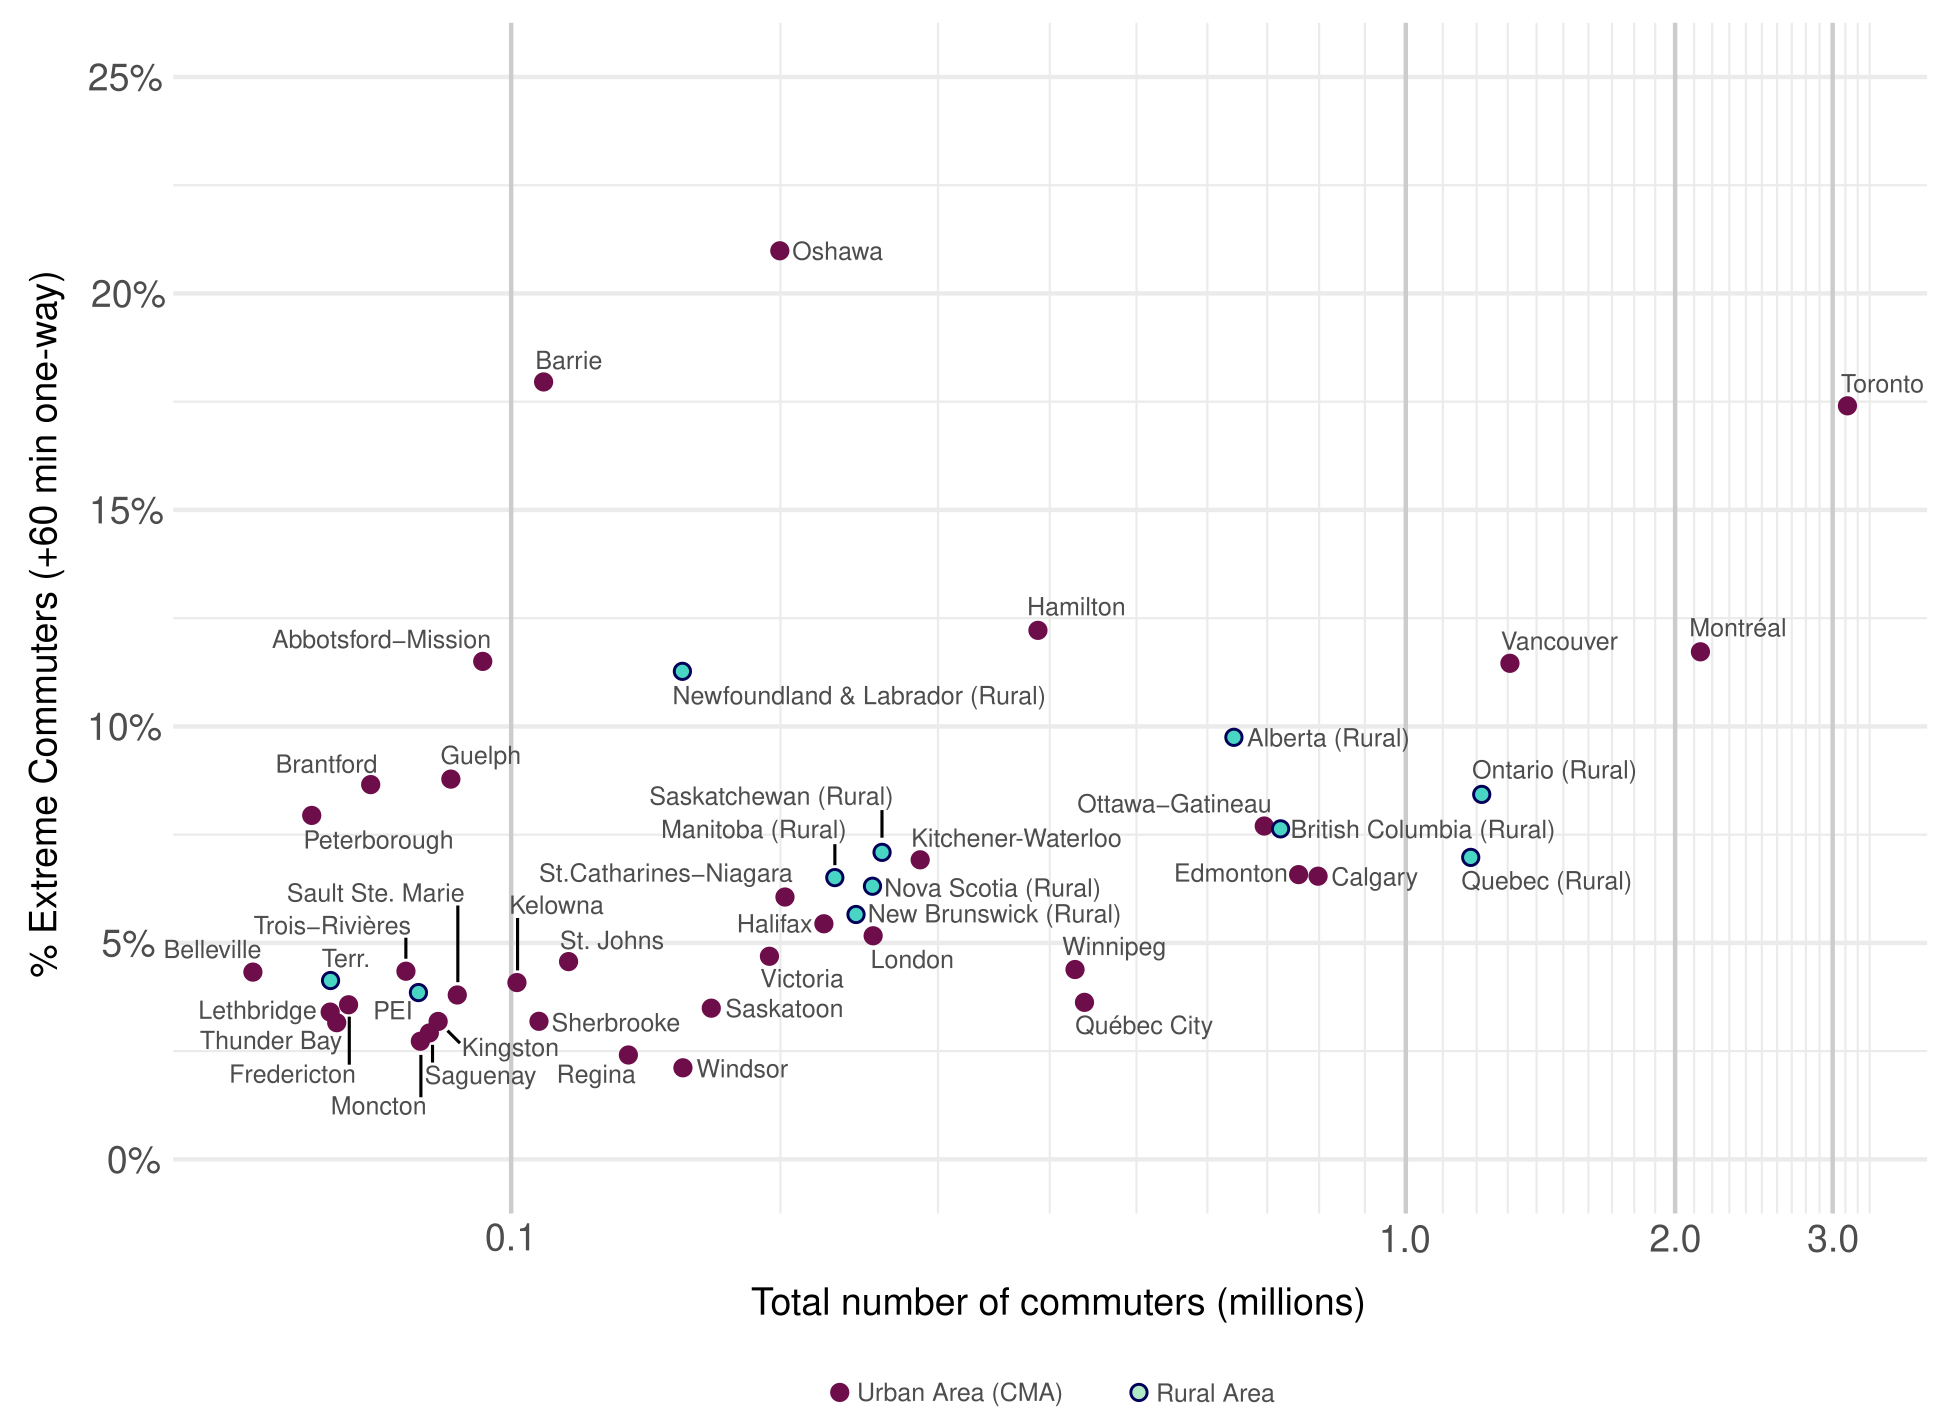
\includegraphics[width=6.5in]{figures/geog_plot_v5.png}}
	\caption{Prevalence of extreme commuting by region in Canada in 2016}
	\label{fig:geog_base}
\end{figure}







\begin{figure}[H]
	\centering
	\makebox[\textwidth][c]{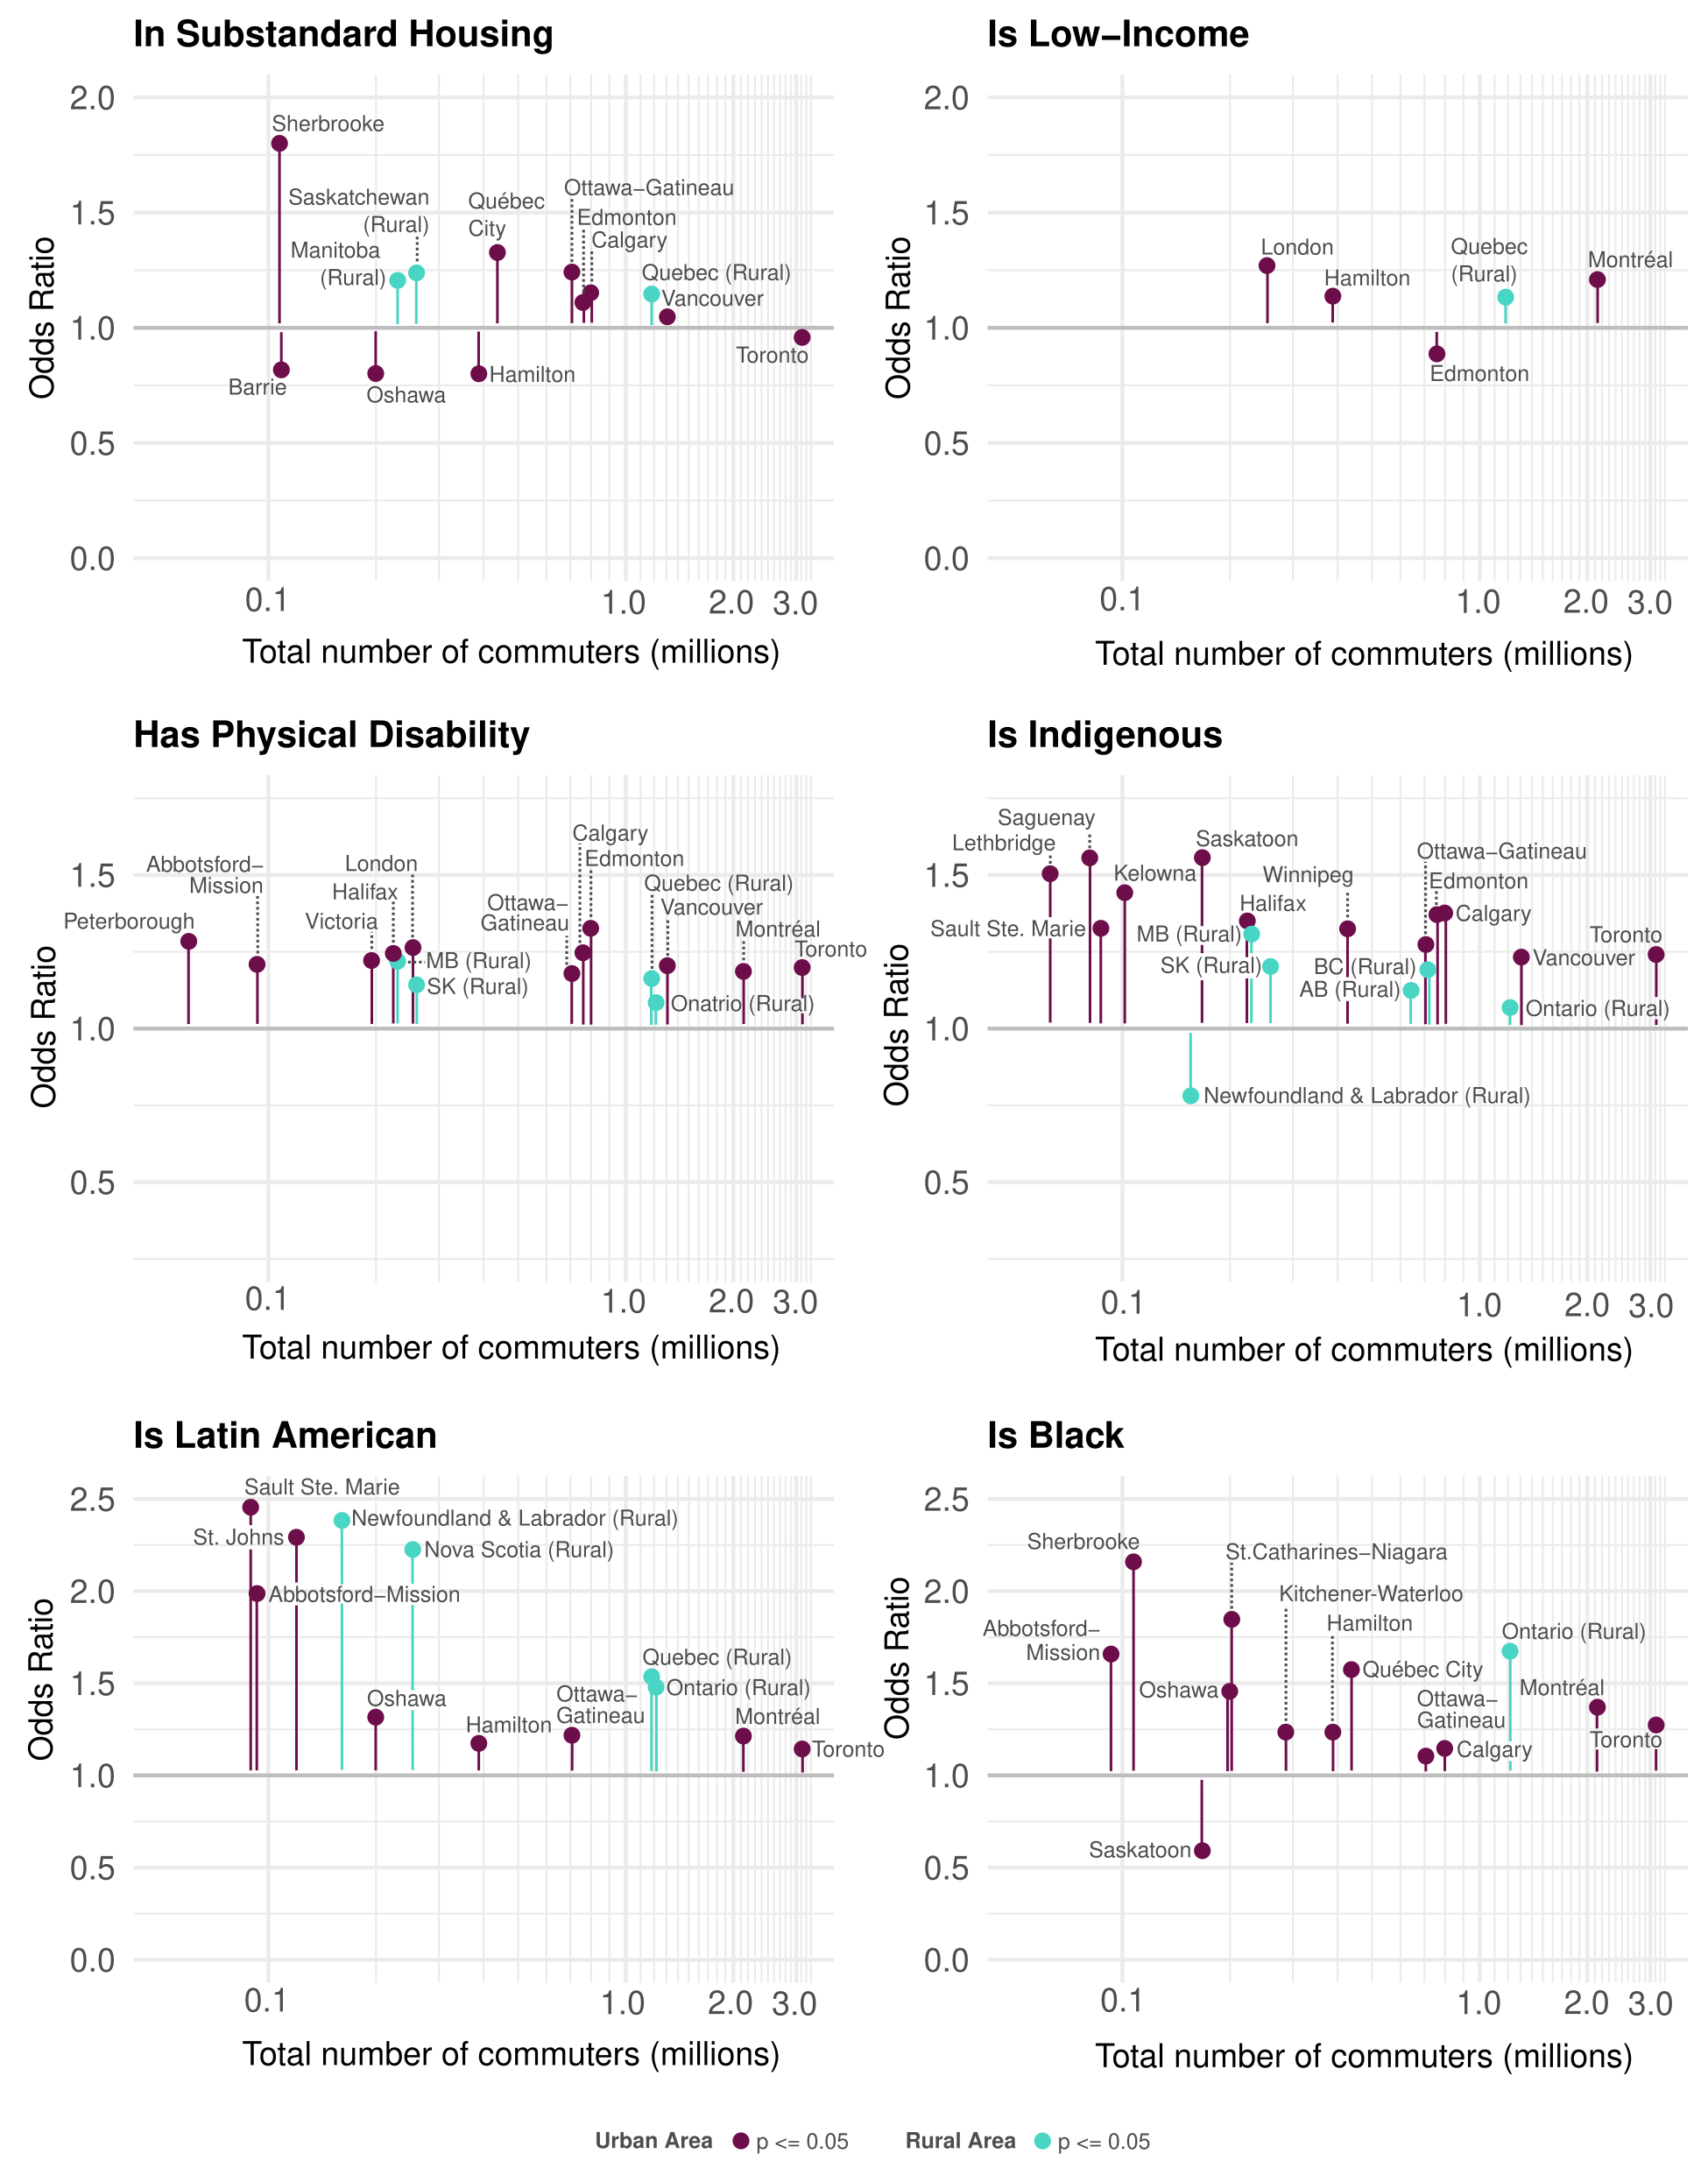
\includegraphics[width=6.5in]{figures/beta_by_geog_v5.png}}
	\caption{Significant Odds Ratios by region for select variables}
	\label{fig:CMA_Results_ORs}
\end{figure}


\section{Conclusions}

Prior to COVID-19, we find that extreme commuting in Canada was more prevalent among socially disadvantaged residents, particularly in major metropolitan areas, mirroring results elsewhere \cite{marion_comparison_2007,bai_exploring_2020}. In Canada, groups over-represented as extreme commuters include people with physical limitations, low-income workers, those in sub-standard housing, transit commuters, and those in trades like mining and agriculture. Our results also offer new insights on transportation assimilation and the immigration effect on commuting \cite{newbold_immigrant_2017,harun_immigrant_2021, Axisa_2012}. We show that the longer an immigrant stays in Canada, the more likely they will become an extreme commuter relative to Canadian-born residents, indicating that immigrants' efforts to attain home ownership are coming at the cost of significant time lost to commuting. 

Even after controlling for other factors, we find extreme commuting is significantly more common among several visible minority groups relative to white commuters, including Black and Indigenous commuters. This suggests that race, or the social and economic forces that act on racialized Canadians but not White Canadians, contribute to inequalities in commuting and in doing so, put racialized Canadians at greater risk of experiencing the negative impacts of excess commuting, from increased divorce rates to worse sleep quality and poorer mental health \cite{hansson_relationship_2011, roberts_its_2011, sandow_til_2019}. And while our national results point to major cities as the primary geographical contexts producing extreme commuting, the racialized inequality in extreme commuting is also significant in several of the country's smaller CMAs and rural areas, particularly for Indigenous and Black commuters (see Figure \ref{fig:CMA_Results_ORs}). Indigenous commuters' challenges with extreme commuting are most severe in places where the urban indigenous population is large, including several small and mid-sized metros and Calgary. Further research is needed to identify why and what can be done about it.

Canadian extreme commuting exhibits patterns similar to extreme commuting in other parts of the global north. Roughly the same proportion of Canadian and European workers travel more than 60 minutes to work \cite{vincent-geslin_determinants_2016}. The proportion of Canadians workers traveling more than 90 minutes is similar to the proportions found in U.S. cities, between two and three percent \cite{marion_comparison_2007}.  Racial differences identified in this study mirror the American experience as well \cite{mclafferty_who_2019,preston_revisiting_2016}. These parallels point to the possibility of similar structural forces contributing to and limiting the extent of extreme commuting across these countries, such as discrimination in housing \cite{murdie2002housing} and employment \cite{galabuzi2006canada,dietz2015skill}. 

Our research does contain several data limitations. Most importantly, we could not control for how often individuals travel to work per week. Extreme commuters may travel to work less frequently, and the COVID-19 pandemic undoubtedly makes this an important consideration for future work. We certainly recommend that future censuses collect information on weekly commute and telecommute frequency. We also could not account for vehicle ownership and availability, as the question is not asked in the Canadian census (we are only able to partly control for this by having a variable for travel mode). Finally, our national scope limits our use of more refined built form statistics, such as detailed measures of transit accessibility. Subsequent work could also explore how the intersections of personal, household, and built form factors contribute to extreme commuting through classification or interaction models. 

On a more fundamental level, we demonstrate that race and immigrant status matters when considering travel behaviour in the Canadian context. Our results do not point to which structural forces or individual preferences may explain the systematic over-representation of visible minorities in extreme commuting across Canada. Future work should examine the social, economic, and geographical forces contributing to the over-representation of racialized Canadians among extreme commuters. If race is such a strong predictor of commute times, it is likely a significant predictor of other transportation measures. Canadian practitioners and academics should include race and immigration status as standard questions on household travel surveys (most regional travel surveys in Canada currently do not include these questions). This will help policymakers identify how and when our transport and land use systems place burdens disproportionately on racialized Canadians, and will hopefully lead to further research identifying what to do about it.  COVID-19 only amplifies the importance of considering race and immigration in travel behaviour, as immigrants and racialized people were more likely to continue traveling by public transit during the crisis \cite{palm_allen21}, and we find that transit riders are over-represented among extreme commuters. Further, extreme transit commutes during the pandemic meant longer periods of potential exposure to infection, while pandemic-induced service cuts risk increasing commute times for these commuters.

Moreover, further research is needed to distinguish between different types of extreme commuting and their respective causes. As extreme commuting is primarily driven by auto and transit modes \cite{marion_comparison_2007, maoh_determinants_2012-1, vincent-geslin_determinants_2016, bai_exploring_2020}, stratified models by each transport mode and more fine grained regional analyses may reveal opportunities for system improvements that reduce some extreme commuters' travel burdens. At the same time, further research is needed to understand the role of personal preferences interacting with complex trade-offs that contribute to these outcomes. Such research could help distinguish between extreme commuting born by inadequate service provision as opposed to personal preferences for larger homes at lower prices or more rural lifestyles. Future work should also seek to identify appropriate thresholds for defining extreme commutes in communities of different sizes. The multiple health, psychological and social impacts of extreme commuting make identifying and addressing unwanted extreme commuting a pressing issue.




\section{Acknowledgements}

The individual file of the long-form 2016 Canadian census was accessed and analyzed at the Research Data Centre (RDC) at the University of Toronto. We additionally would like to thank the staff at the RDC for their help and support in accessing data and releasing results. The first author is also thankful for a graduate scholarship from the Social Sciences and Humanities Research Council of Canada. The second and fourth authors are supported by funding from the Social Sciences and Humanities Research Council’s partnership grant: Mobilizing justice: towards evidence-based transportation equity policy.




\section*{Appendix}

Local accessibility measures were derived from the Proximity Measures Database (PMD) developed by \citeA{statistics_canada_proximity_2020}. Specifically, we generate an overall index based on proximity measures for the eight destinations noted in Table \ref{table:pmd} released at the dissemination block level. Each indicator in the PMB is released on a scale from 0 to 1, where a 0 is when there are no destinations within the network distance noted in Table \ref{table:pmd}, and a 1 is the highest value across all of Canada. All eight indicators were summed and then scaled into a standardized score prior to inputting into the cluster analysis.

\begin{table}[h]
	\small
	\centering
	\caption{{Destination types and network distances used to measure local accessibility}}
	\label{table:pmd}
	\begin{tabular}{lll}
		\hline
		\textbf{Destination}    & \textbf{Network Distance}   \\ \hline
		Grocery stores & 1km \\
		Health care & 3km \\
		Pharmacies & 1km \\
		Child care & 1.5km \\
		Primary education & 1.5km \\
		Secondary education & 1.5km \\
		Neighbourhood parks & 1km \\
		Libraries & 1.5km \\ 
		\hline
	\end{tabular}
\end{table}
	

\renewcommand{\baselinestretch}{1.1} 

\bibliographystyle{apacite}
\bibliography{references.bib}





\end{document}